\documentclass[]{article}
\usepackage{lmodern}
\usepackage{amssymb,amsmath}
\usepackage{ifxetex,ifluatex}
\usepackage{fixltx2e} % provides \textsubscript
\ifnum 0\ifxetex 1\fi\ifluatex 1\fi=0 % if pdftex
  \usepackage[T1]{fontenc}
  \usepackage[utf8]{inputenc}
\else % if luatex or xelatex
  \ifxetex
    \usepackage{mathspec}
  \else
    \usepackage{fontspec}
  \fi
  \defaultfontfeatures{Ligatures=TeX,Scale=MatchLowercase}
\fi
% use upquote if available, for straight quotes in verbatim environments
\IfFileExists{upquote.sty}{\usepackage{upquote}}{}
% use microtype if available
\IfFileExists{microtype.sty}{%
\usepackage{microtype}
\UseMicrotypeSet[protrusion]{basicmath} % disable protrusion for tt fonts
}{}
\usepackage[margin=1in]{geometry}
\usepackage{hyperref}
\hypersetup{unicode=true,
            pdftitle={Devil's Advocacy},
            pdfauthor={Jon Minton},
            pdfborder={0 0 0},
            breaklinks=true}
\urlstyle{same}  % don't use monospace font for urls
\usepackage{color}
\usepackage{fancyvrb}
\newcommand{\VerbBar}{|}
\newcommand{\VERB}{\Verb[commandchars=\\\{\}]}
\DefineVerbatimEnvironment{Highlighting}{Verbatim}{commandchars=\\\{\}}
% Add ',fontsize=\small' for more characters per line
\usepackage{framed}
\definecolor{shadecolor}{RGB}{248,248,248}
\newenvironment{Shaded}{\begin{snugshade}}{\end{snugshade}}
\newcommand{\KeywordTok}[1]{\textcolor[rgb]{0.13,0.29,0.53}{\textbf{#1}}}
\newcommand{\DataTypeTok}[1]{\textcolor[rgb]{0.13,0.29,0.53}{#1}}
\newcommand{\DecValTok}[1]{\textcolor[rgb]{0.00,0.00,0.81}{#1}}
\newcommand{\BaseNTok}[1]{\textcolor[rgb]{0.00,0.00,0.81}{#1}}
\newcommand{\FloatTok}[1]{\textcolor[rgb]{0.00,0.00,0.81}{#1}}
\newcommand{\ConstantTok}[1]{\textcolor[rgb]{0.00,0.00,0.00}{#1}}
\newcommand{\CharTok}[1]{\textcolor[rgb]{0.31,0.60,0.02}{#1}}
\newcommand{\SpecialCharTok}[1]{\textcolor[rgb]{0.00,0.00,0.00}{#1}}
\newcommand{\StringTok}[1]{\textcolor[rgb]{0.31,0.60,0.02}{#1}}
\newcommand{\VerbatimStringTok}[1]{\textcolor[rgb]{0.31,0.60,0.02}{#1}}
\newcommand{\SpecialStringTok}[1]{\textcolor[rgb]{0.31,0.60,0.02}{#1}}
\newcommand{\ImportTok}[1]{#1}
\newcommand{\CommentTok}[1]{\textcolor[rgb]{0.56,0.35,0.01}{\textit{#1}}}
\newcommand{\DocumentationTok}[1]{\textcolor[rgb]{0.56,0.35,0.01}{\textbf{\textit{#1}}}}
\newcommand{\AnnotationTok}[1]{\textcolor[rgb]{0.56,0.35,0.01}{\textbf{\textit{#1}}}}
\newcommand{\CommentVarTok}[1]{\textcolor[rgb]{0.56,0.35,0.01}{\textbf{\textit{#1}}}}
\newcommand{\OtherTok}[1]{\textcolor[rgb]{0.56,0.35,0.01}{#1}}
\newcommand{\FunctionTok}[1]{\textcolor[rgb]{0.00,0.00,0.00}{#1}}
\newcommand{\VariableTok}[1]{\textcolor[rgb]{0.00,0.00,0.00}{#1}}
\newcommand{\ControlFlowTok}[1]{\textcolor[rgb]{0.13,0.29,0.53}{\textbf{#1}}}
\newcommand{\OperatorTok}[1]{\textcolor[rgb]{0.81,0.36,0.00}{\textbf{#1}}}
\newcommand{\BuiltInTok}[1]{#1}
\newcommand{\ExtensionTok}[1]{#1}
\newcommand{\PreprocessorTok}[1]{\textcolor[rgb]{0.56,0.35,0.01}{\textit{#1}}}
\newcommand{\AttributeTok}[1]{\textcolor[rgb]{0.77,0.63,0.00}{#1}}
\newcommand{\RegionMarkerTok}[1]{#1}
\newcommand{\InformationTok}[1]{\textcolor[rgb]{0.56,0.35,0.01}{\textbf{\textit{#1}}}}
\newcommand{\WarningTok}[1]{\textcolor[rgb]{0.56,0.35,0.01}{\textbf{\textit{#1}}}}
\newcommand{\AlertTok}[1]{\textcolor[rgb]{0.94,0.16,0.16}{#1}}
\newcommand{\ErrorTok}[1]{\textcolor[rgb]{0.64,0.00,0.00}{\textbf{#1}}}
\newcommand{\NormalTok}[1]{#1}
\usepackage{graphicx,grffile}
\makeatletter
\def\maxwidth{\ifdim\Gin@nat@width>\linewidth\linewidth\else\Gin@nat@width\fi}
\def\maxheight{\ifdim\Gin@nat@height>\textheight\textheight\else\Gin@nat@height\fi}
\makeatother
% Scale images if necessary, so that they will not overflow the page
% margins by default, and it is still possible to overwrite the defaults
% using explicit options in \includegraphics[width, height, ...]{}
\setkeys{Gin}{width=\maxwidth,height=\maxheight,keepaspectratio}
\IfFileExists{parskip.sty}{%
\usepackage{parskip}
}{% else
\setlength{\parindent}{0pt}
\setlength{\parskip}{6pt plus 2pt minus 1pt}
}
\setlength{\emergencystretch}{3em}  % prevent overfull lines
\providecommand{\tightlist}{%
  \setlength{\itemsep}{0pt}\setlength{\parskip}{0pt}}
\setcounter{secnumdepth}{0}
% Redefines (sub)paragraphs to behave more like sections
\ifx\paragraph\undefined\else
\let\oldparagraph\paragraph
\renewcommand{\paragraph}[1]{\oldparagraph{#1}\mbox{}}
\fi
\ifx\subparagraph\undefined\else
\let\oldsubparagraph\subparagraph
\renewcommand{\subparagraph}[1]{\oldsubparagraph{#1}\mbox{}}
\fi

%%% Use protect on footnotes to avoid problems with footnotes in titles
\let\rmarkdownfootnote\footnote%
\def\footnote{\protect\rmarkdownfootnote}

%%% Change title format to be more compact
\usepackage{titling}

% Create subtitle command for use in maketitle
\providecommand{\subtitle}[1]{
  \posttitle{
    \begin{center}\large#1\end{center}
    }
}

\setlength{\droptitle}{-2em}

  \title{Devil's Advocacy}
    \pretitle{\vspace{\droptitle}\centering\huge}
  \posttitle{\par}
    \author{Jon Minton}
    \preauthor{\centering\large\emph}
  \postauthor{\par}
      \predate{\centering\large\emph}
  \postdate{\par}
    \date{15 August 2019}


\begin{document}
\maketitle

\section{Introduction}\label{introduction}

The Bayes Factor approach has been used to test for both the likelihood
and magnitude of various proposed levels of life expectancy slowdown. By
assuming that 1990-2012 is the `before slowdown' period and the years
after the `after-slowdown' period. After combining five successive
observations, annual changes in life expectancy, a Bayes Factor of
around 1.003 was produced for a proposed slowdown of around 77\% of
previous levels.

The exercise followed from trying to formalise an intuitive `reading' of
the life expectancy series for the UK, which is that the curve in life
expectancy looks much `flatter' after around 2012 than from 1990 up to
that year. Five observations, annual changes since 2012, were used to
investivate the relative likelihood of a slowdown compared with no
slowdown.

However, looking at the time series of life expectancy over time, there
appears to be another way of interpreting the series. This is that life
expectancy gains briefly \emph{increased} after the 2008 recession,
before \emph{returning to their previous trajectory} in the last few
years. Graphically, the two proposed interpretations can be represented
as follows

\begin{Shaded}
\begin{Highlighting}[]
\KeywordTok{source}\NormalTok{(}\StringTok{"scripts/load_packages_and_functions.R"}\NormalTok{)}

\NormalTok{e0_uk <-}\StringTok{ }\KeywordTok{read_csv}\NormalTok{(}\StringTok{"data/e0_uk.csv"}\NormalTok{)}
\end{Highlighting}
\end{Shaded}

\begin{verbatim}
## Parsed with column specification:
## cols(
##   year = col_double(),
##   sex = col_character(),
##   e0 = col_double()
## )
\end{verbatim}

The Slowdown interpretation, which the majority of research to date has
focused on, proposes that, after a certain date (2012), the rate of
annual improvement in life expectancy has slowed. Graphically, this is
presented as two discontinuous lines of life expectancy over time, a
higher improvement rate period, covering 1990-2012, and a lower
improvement (or even zero improvement) rate period, for those years
after 2012. This looks as follows:

\begin{Shaded}
\begin{Highlighting}[]
\NormalTok{e0_uk }\OperatorTok\StringTok{ }
\StringTok{  }\KeywordTok{filter}\NormalTok{(year }\OperatorTok{>=}\StringTok{ }\DecValTok{1990}\NormalTok{) }\OperatorTok\StringTok{ }
\StringTok{  }\KeywordTok{mutate}\NormalTok{(}\DataTypeTok{period =} \KeywordTok{case_when}\NormalTok{(}
\NormalTok{    year }\OperatorTok{<=}\StringTok{ }\DecValTok{2012}     \OperatorTok{~}\StringTok{ "Before slowdown"}\NormalTok{,}
\NormalTok{    year }\OperatorTok{>}\StringTok{ }\DecValTok{2012}      \OperatorTok{~}\StringTok{ "After slowdown"}
\NormalTok{  )) }\OperatorTok\StringTok{ }
\StringTok{  }\KeywordTok{ggplot}\NormalTok{(}\KeywordTok{aes}\NormalTok{(}\DataTypeTok{x =}\NormalTok{ year, }\DataTypeTok{y =}\NormalTok{ e0, }\DataTypeTok{group =}\NormalTok{ sex, }\DataTypeTok{colour =}\NormalTok{ sex, }\DataTypeTok{linetype =}\NormalTok{ sex)) }\OperatorTok{+}
\StringTok{  }\KeywordTok{geom_point}\NormalTok{() }\OperatorTok{+}\StringTok{ }
\StringTok{  }\KeywordTok{stat_smooth}\NormalTok{(}\KeywordTok{aes}\NormalTok{(}\DataTypeTok{x =}\NormalTok{ year, }\DataTypeTok{y =}\NormalTok{ e0, }\DataTypeTok{group =} \KeywordTok{paste0}\NormalTok{(sex, period), }\DataTypeTok{colour =}\NormalTok{ sex, }\DataTypeTok{linetype =}\NormalTok{ sex), }
              \DataTypeTok{method =} \StringTok{"lm"}\NormalTok{, }\DataTypeTok{se =}\NormalTok{ F) }\OperatorTok{+}\StringTok{ }
\StringTok{  }\KeywordTok{labs}\NormalTok{(}\DataTypeTok{x =} \StringTok{"Year"}\NormalTok{, }\DataTypeTok{y =} \StringTok{"Period life expectancy at birth"}\NormalTok{,}
       \DataTypeTok{title =} \StringTok{"Slowdown interpretation"}\NormalTok{,}
       \DataTypeTok{caption =} \StringTok{"Sources: HMD; ONS for 2017"}\NormalTok{) }\OperatorTok{+}\StringTok{ }
\StringTok{  }\KeywordTok{geom_vline}\NormalTok{(}\DataTypeTok{xintercept =} \DecValTok{2012}\NormalTok{) }\OperatorTok{+}\StringTok{ }
\StringTok{  }\KeywordTok{annotate}\NormalTok{(}\DataTypeTok{geom =} \StringTok{"text"}\NormalTok{, }\DataTypeTok{x =} \DecValTok{2012}\NormalTok{, }\DataTypeTok{y =} \DecValTok{75}\NormalTok{, }\DataTypeTok{label =} \StringTok{"2012"}\NormalTok{, }\DataTypeTok{colour =} \StringTok{"darkred"}\NormalTok{, }\DataTypeTok{angle =} \DecValTok{90}\NormalTok{) }\OperatorTok{+}\StringTok{ }
\StringTok{  }\KeywordTok{scale_x_continuous}\NormalTok{(}\DataTypeTok{breaks =} \KeywordTok{seq}\NormalTok{(}\DecValTok{1990}\NormalTok{, }\DecValTok{2015}\NormalTok{, }\DataTypeTok{by =} \DecValTok{5}\NormalTok{))}
\end{Highlighting}
\end{Shaded}

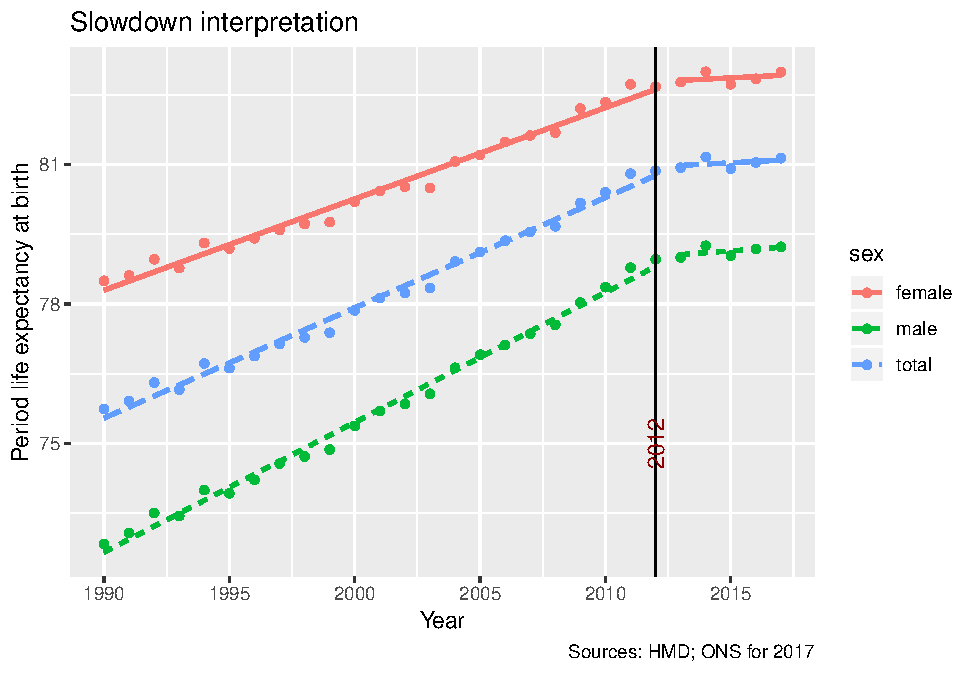
\includegraphics{devils_advocacy_files/figure-latex/unnamed-chunk-2-1.pdf}

Another possible interpretation of the same data is that the last period
is broadly typical of improvement rates over the whole period. Instead,
the `atypical' period was in the years immediately following the 2008
recession, during which life expectancy improvement rates briefly
\emph{increased}. Under this interpretation, the apparent flattening in
the curve is due to a relatively typical period of life expectancy
improvmeent following an atypically \emph{good} period of improvement,
rather than being a genuine slowdown from a typical to a slow
improvement period. Graphically, this alternative reading of the data
looks as follows:

\begin{Shaded}
\begin{Highlighting}[]
\NormalTok{e0_uk }\OperatorTok\StringTok{ }
\StringTok{  }\KeywordTok{filter}\NormalTok{(year }\OperatorTok{>=}\StringTok{ }\DecValTok{1990}\NormalTok{) }\OperatorTok\StringTok{ }
\StringTok{  }\KeywordTok{mutate}\NormalTok{(}\DataTypeTok{period =} \KeywordTok{case_when}\NormalTok{(}
    \KeywordTok{between}\NormalTok{(year, }\DecValTok{2009}\NormalTok{, }\DecValTok{2014}\NormalTok{) }\OperatorTok{~}\StringTok{ "GFC Bump"}\NormalTok{,}
    \OtherTok{TRUE}                      \OperatorTok{~}\StringTok{ "Improvement as usual"}
\NormalTok{  )) }\OperatorTok\StringTok{ }
\StringTok{  }\KeywordTok{ggplot}\NormalTok{(}\KeywordTok{aes}\NormalTok{(}\DataTypeTok{x =}\NormalTok{ year, }\DataTypeTok{y =}\NormalTok{ e0, }\DataTypeTok{group =}\NormalTok{ sex, }\DataTypeTok{colour =}\NormalTok{ sex, }\DataTypeTok{linetype =}\NormalTok{ sex)) }\OperatorTok{+}
\StringTok{  }\KeywordTok{geom_point}\NormalTok{() }\OperatorTok{+}\StringTok{ }
\StringTok{  }\KeywordTok{stat_smooth}\NormalTok{(}\KeywordTok{aes}\NormalTok{(}\DataTypeTok{x =}\NormalTok{ year, }\DataTypeTok{y =}\NormalTok{ e0, }\DataTypeTok{group =} \KeywordTok{paste0}\NormalTok{(sex, period), }\DataTypeTok{colour =}\NormalTok{ sex, }\DataTypeTok{linetype =}\NormalTok{ sex), }
              \DataTypeTok{method =} \StringTok{"lm"}\NormalTok{, }\DataTypeTok{se =}\NormalTok{ F) }\OperatorTok{+}\StringTok{ }
\StringTok{  }\KeywordTok{labs}\NormalTok{(}\DataTypeTok{x =} \StringTok{"Year"}\NormalTok{, }\DataTypeTok{y =} \StringTok{"Period life expectancy at birth"}\NormalTok{,}
       \DataTypeTok{title =} \StringTok{"GFC Bump Interpretation"}\NormalTok{,}
       \DataTypeTok{caption =} \StringTok{"Sources: HMD; ONS for 2017"}\NormalTok{) }\OperatorTok{+}\StringTok{ }
\StringTok{  }\KeywordTok{geom_vline}\NormalTok{(}\DataTypeTok{xintercept =} \DecValTok{2009}\NormalTok{) }\OperatorTok{+}\StringTok{ }
\StringTok{  }\KeywordTok{geom_vline}\NormalTok{(}\DataTypeTok{xintercept =} \DecValTok{2014}\NormalTok{) }\OperatorTok{+}\StringTok{ }
\StringTok{  }\KeywordTok{scale_x_continuous}\NormalTok{(}\DataTypeTok{breaks =} \KeywordTok{seq}\NormalTok{(}\DecValTok{1990}\NormalTok{, }\DecValTok{2015}\NormalTok{, }\DataTypeTok{by =} \DecValTok{5}\NormalTok{))}
\end{Highlighting}
\end{Shaded}

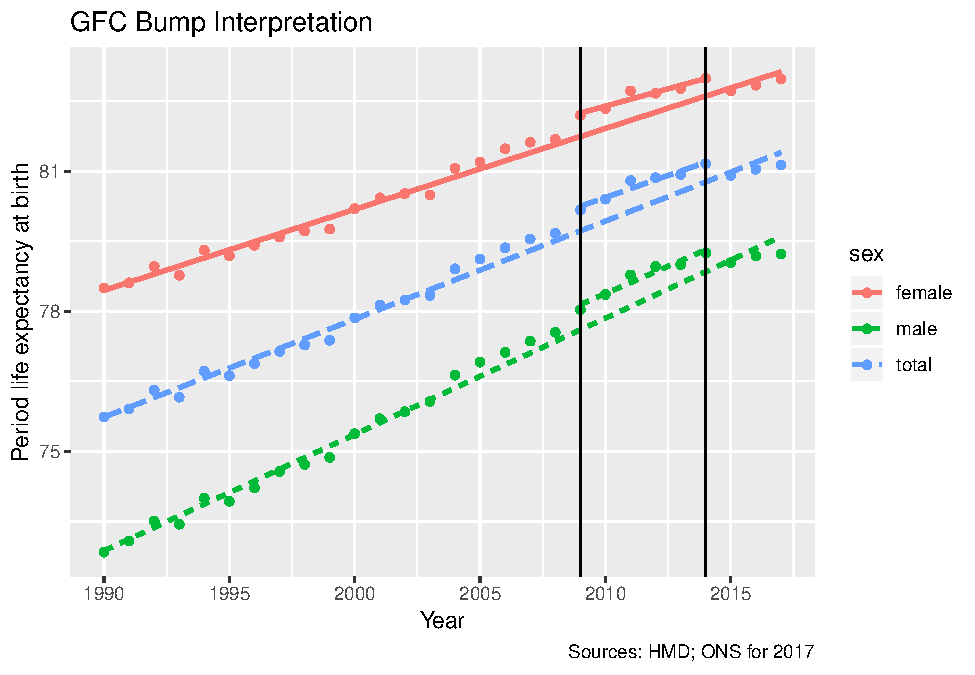
\includegraphics{devils_advocacy_files/figure-latex/unnamed-chunk-3-1.pdf}

Both of these interpetations are based on the same number of continuous
observations of values that appear discordant with the overall series.
Both interpretations also appear theoretically justifiable: Whereas the
proposed mechanism for the slowdown interpretation is that Austerity
implemented in the post-GFC period has led to a substantial
deterioration of health and social care services, with consequent
adverse effects on population health, the proposed mechanism for the GFC
bump would be that reductions in dependable disposible income would lead
to, on the average, a higher proportion of personal spend being
salugenic rather than pathogenic. The most obvious example of this would
be if, as a result of having less disposible income, the UK population
cannot afford to drive as much, and so faces a reduced exposure to
vehicle-related mortality. Another example would include reduced alcohol
consumption, and so a reduced hazard of alcohol-related mortality. In
the conclusion of this document, some of the testable implications of
the GFC `bump' hypothesis will be considered further.

\section{Graphs of annual change}\label{graphs-of-annual-change}

Both the Slowdown and the GFC Bump interpretations can be expressed
through graphs of annual changes in life expectancy, rather than life
expectancy alone. In both graphs of annual change, points are added to
some line segments. These indicate the points that are considered
`atypical' from the perspective of the interpretation under
consideration.

The graph showing annual changes under the GFC Bump interpretation is
shown in the following:

\begin{Shaded}
\begin{Highlighting}[]
\NormalTok{e0_uk }\OperatorTok\StringTok{ }
\StringTok{  }\KeywordTok{group_by}\NormalTok{(sex) }\OperatorTok\StringTok{ }
\StringTok{  }\KeywordTok{arrange}\NormalTok{(year) }\OperatorTok\StringTok{ }
\StringTok{  }\KeywordTok{mutate}\NormalTok{(}\DataTypeTok{ch_e0 =}\NormalTok{ e0 }\OperatorTok{-}\StringTok{ }\KeywordTok{lag}\NormalTok{(e0)) }\OperatorTok\StringTok{ }
\StringTok{  }\KeywordTok{filter}\NormalTok{(year }\OperatorTok{>=}\StringTok{ }\DecValTok{1990}\NormalTok{) }\OperatorTok\StringTok{ }
\StringTok{  }\KeywordTok{ggplot}\NormalTok{(}\KeywordTok{aes}\NormalTok{(}\DataTypeTok{x =}\NormalTok{ year, }\DataTypeTok{y =}\NormalTok{ ch_e0)) }\OperatorTok{+}
\StringTok{  }\KeywordTok{geom_line}\NormalTok{() }\OperatorTok{+}\StringTok{ }
\StringTok{  }\KeywordTok{geom_point}\NormalTok{(}\KeywordTok{aes}\NormalTok{(}\DataTypeTok{x =}\NormalTok{ year, }\DataTypeTok{y=}\NormalTok{ ch_e0), }\DataTypeTok{inherit.aes =} \OtherTok{FALSE}\NormalTok{, }
             \DataTypeTok{data =}\NormalTok{ . }\OperatorTok\StringTok{ }\KeywordTok{filter}\NormalTok{(}\KeywordTok{between}\NormalTok{(year, }\DecValTok{2009}\NormalTok{, }\DecValTok{2013}\NormalTok{))}
\NormalTok{  ) }\OperatorTok{+}
\StringTok{  }\KeywordTok{labs}\NormalTok{(}\DataTypeTok{x =} \StringTok{"Year"}\NormalTok{, }\DataTypeTok{y =} \StringTok{"Change in life expectancy from previous year"}\NormalTok{,}
       \DataTypeTok{title =} \StringTok{"Annual changes in life expectancy in the UK since 1990"}\NormalTok{,}
       \DataTypeTok{caption =} \StringTok{"Sources: HMD; ONS for 2017"}\NormalTok{) }\OperatorTok{+}\StringTok{ }
\StringTok{  }\KeywordTok{geom_vline}\NormalTok{(}\DataTypeTok{xintercept =} \DecValTok{2008}\NormalTok{) }\OperatorTok{+}\StringTok{   }\KeywordTok{geom_vline}\NormalTok{(}\DataTypeTok{xintercept =} \DecValTok{2014}\NormalTok{) }\OperatorTok{+}\StringTok{ }
\StringTok{  }\KeywordTok{scale_x_continuous}\NormalTok{(}\DataTypeTok{breaks =} \KeywordTok{seq}\NormalTok{(}\DecValTok{1990}\NormalTok{, }\DecValTok{2015}\NormalTok{, }\DataTypeTok{by =} \DecValTok{5}\NormalTok{)) }\OperatorTok{+}\StringTok{ }
\StringTok{  }\KeywordTok{geom_hline}\NormalTok{(}\DataTypeTok{yintercept =} \DecValTok{0}\NormalTok{) }\OperatorTok{+}
\StringTok{  }\KeywordTok{facet_grid}\NormalTok{(sex }\OperatorTok{~}\StringTok{ }\NormalTok{.) }\OperatorTok{+}\StringTok{ }
\StringTok{  }\KeywordTok{theme_minimal}\NormalTok{()}
\end{Highlighting}
\end{Shaded}

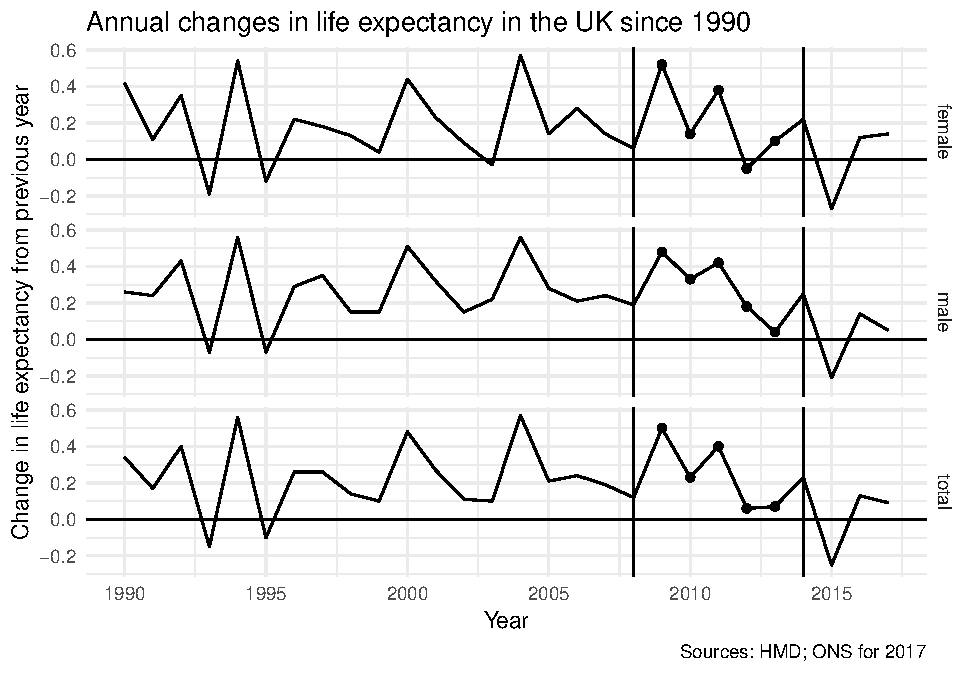
\includegraphics{devils_advocacy_files/figure-latex/unnamed-chunk-4-1.pdf}

Of these five observations, the last two do not like particular `good'
years, with a small decline in life expectancy observed for one year for
females. Also the improvement years are not higher than those observed
since 1990 previously. However, the use of five observations makes
meaningful comparison with the previous exercise more straightforward.

Let's now calculate the average change and standard deviation around
this for the series excluding these five points. This will form the new
Null model specification.

\begin{Shaded}
\begin{Highlighting}[]
\NormalTok{devils_summaries <-}\StringTok{ }
\StringTok{  }\NormalTok{e0_uk }\OperatorTok\StringTok{ }
\StringTok{    }\KeywordTok{group_by}\NormalTok{(sex) }\OperatorTok\StringTok{ }
\StringTok{    }\KeywordTok{arrange}\NormalTok{(year) }\OperatorTok\StringTok{ }
\StringTok{    }\KeywordTok{mutate}\NormalTok{(}\DataTypeTok{ch_e0 =}\NormalTok{ e0 }\OperatorTok{-}\StringTok{ }\KeywordTok{lag}\NormalTok{(e0)) }\OperatorTok\StringTok{ }
\StringTok{    }\KeywordTok{filter}\NormalTok{(year }\OperatorTok{>=}\StringTok{ }\DecValTok{1990}\NormalTok{) }\OperatorTok
\StringTok{    }\KeywordTok{filter}\NormalTok{(}\OperatorTok{!}\KeywordTok{between}\NormalTok{(year, }\DecValTok{2009}\NormalTok{, }\DecValTok{2013}\NormalTok{)) }\OperatorTok\StringTok{ }
\StringTok{    }\KeywordTok{group_by}\NormalTok{(sex) }\OperatorTok\StringTok{ }
\StringTok{    }\KeywordTok{summarise}\NormalTok{(}\DataTypeTok{mu_ch =} \KeywordTok{mean}\NormalTok{(ch_e0), }
              \DataTypeTok{var_ch =} \KeywordTok{var}\NormalTok{(ch_e0)}
\NormalTok{    )}

\NormalTok{devils_summaries}
\end{Highlighting}
\end{Shaded}

\begin{verbatim}
## # A tibble: 3 x 3
##   sex    mu_ch var_ch
##   <chr>  <dbl>  <dbl>
## 1 female 0.166 0.0445
## 2 male   0.226 0.0364
## 3 total  0.194 0.0404
\end{verbatim}

The means are somewhat lower than previously calculated (under the
Slowdown interpretation); the variances are similar

\section{Bayes factors}\label{bayes-factors}

As when evaluating the Slowdown interpretion, the GFC Bump
interpretation compares the relative likelihood of the assumption that
life expectancy changes in the `atypical' period were different from
those in the `typical' period, to the assumption that they were the
same. Unlike with the Slowdown interpretation, the proposed differences
are all higher rather than lower than the `typical' period, with
proposed improvement levels between 100\% and 200\% of their `typical
period' levels.

Using the first year of the atypical period under the GFC Bump
interpretion alone, the Bayes Factor schedule looks as follows:

\begin{Shaded}
\begin{Highlighting}[]
\NormalTok{e0_uk_bf <-}\StringTok{ }
\StringTok{  }\NormalTok{e0_uk }\OperatorTok\StringTok{ }
\StringTok{  }\KeywordTok{group_by}\NormalTok{(sex) }\OperatorTok\StringTok{ }
\StringTok{  }\KeywordTok{arrange}\NormalTok{(year) }\OperatorTok\StringTok{ }
\StringTok{  }\KeywordTok{mutate}\NormalTok{(}\DataTypeTok{ch_e0 =}\NormalTok{ e0 }\OperatorTok{-}\StringTok{ }\KeywordTok{lag}\NormalTok{(e0)) }\OperatorTok\StringTok{ }
\StringTok{  }\KeywordTok{filter}\NormalTok{(year }\OperatorTok{>=}\StringTok{ }\DecValTok{1990}\NormalTok{) }\OperatorTok
\StringTok{  }\KeywordTok{nest}\NormalTok{() }\OperatorTok\StringTok{ }
\StringTok{  }\KeywordTok{crossing}\NormalTok{(}\DataTypeTok{drop_end =} \DecValTok{2008}\OperatorTok{:}\DecValTok{2013}\NormalTok{) }\OperatorTok\StringTok{ }
\StringTok{  }\KeywordTok{mutate}\NormalTok{(}
    \DataTypeTok{bayes_df =} \KeywordTok{map2}\NormalTok{(}
\NormalTok{      drop_end, data, }\OperatorTok{~}\KeywordTok{calc_devils_bayes_factors}\NormalTok{(}\DataTypeTok{drop_period =} \KeywordTok{c}\NormalTok{(}\DecValTok{2008}\NormalTok{, .x), }\DataTypeTok{full_period =} \KeywordTok{c}\NormalTok{(}\DecValTok{1990}\NormalTok{, }\DecValTok{2016}\NormalTok{), }\DataTypeTok{outcome_var =}\NormalTok{ ch_e0, }\DataTypeTok{dta =}\NormalTok{ .y)}
\NormalTok{    )}
\NormalTok{  ) }\OperatorTok
\StringTok{  }\KeywordTok{select}\NormalTok{(sex, drop_end, bayes_df) }\OperatorTok\StringTok{ }
\StringTok{  }\KeywordTok{unnest}\NormalTok{() }\OperatorTok\StringTok{ }
\StringTok{  }\KeywordTok{mutate}\NormalTok{(}
    \DataTypeTok{period =} \KeywordTok{paste0}\NormalTok{(}\StringTok{"2008-"}\NormalTok{, }\KeywordTok{str_sub}\NormalTok{(drop_end, }\DecValTok{3}\NormalTok{,}\DecValTok{4}\NormalTok{))}
\NormalTok{  ) }
\end{Highlighting}
\end{Shaded}

\begin{verbatim}
## Joining, by = c("year", "e0", "ch_e0")
## Joining, by = c("year", "e0", "ch_e0")
## Joining, by = c("year", "e0", "ch_e0")
## Joining, by = c("year", "e0", "ch_e0")
## Joining, by = c("year", "e0", "ch_e0")
## Joining, by = c("year", "e0", "ch_e0")
## Joining, by = c("year", "e0", "ch_e0")
## Joining, by = c("year", "e0", "ch_e0")
## Joining, by = c("year", "e0", "ch_e0")
## Joining, by = c("year", "e0", "ch_e0")
## Joining, by = c("year", "e0", "ch_e0")
## Joining, by = c("year", "e0", "ch_e0")
## Joining, by = c("year", "e0", "ch_e0")
## Joining, by = c("year", "e0", "ch_e0")
## Joining, by = c("year", "e0", "ch_e0")
## Joining, by = c("year", "e0", "ch_e0")
## Joining, by = c("year", "e0", "ch_e0")
## Joining, by = c("year", "e0", "ch_e0")
\end{verbatim}

First year only

\begin{Shaded}
\begin{Highlighting}[]
\NormalTok{e0_uk_bf }\OperatorTok\StringTok{ }
\StringTok{  }\KeywordTok{filter}\NormalTok{(period }\OperatorTok{==}\StringTok{ "2008-09"}\NormalTok{) }\OperatorTok\StringTok{ }
\StringTok{  }\KeywordTok{mutate}\NormalTok{(}\DataTypeTok{perc =} \DecValTok{100} \OperatorTok{*}\StringTok{ }\NormalTok{perc) }\OperatorTok\StringTok{ }
\StringTok{  }\KeywordTok{ggplot}\NormalTok{(}\KeywordTok{aes}\NormalTok{(}\DataTypeTok{x =}\NormalTok{ perc, }\DataTypeTok{y =}\NormalTok{ bayes_factor)) }\OperatorTok{+}
\StringTok{  }\KeywordTok{geom_line}\NormalTok{() }\OperatorTok{+}\StringTok{ }
\StringTok{  }\KeywordTok{geom_ribbon}\NormalTok{(}\KeywordTok{aes}\NormalTok{(}\DataTypeTok{ymin =} \DecValTok{1}\NormalTok{, }\DataTypeTok{x =}\NormalTok{ perc, }\DataTypeTok{ymax =}\NormalTok{ bayes_factor,}\DataTypeTok{fill =}\NormalTok{ is_pos), }
              \DataTypeTok{data =}\NormalTok{ e0_uk_bf }\OperatorTok\StringTok{ }
\StringTok{                }\KeywordTok{filter}\NormalTok{(period }\OperatorTok{==}\StringTok{ "2008-09"}\NormalTok{) }\OperatorTok\StringTok{ }
\StringTok{                }\KeywordTok{mutate}\NormalTok{(}\DataTypeTok{perc =} \DecValTok{100} \OperatorTok{*}\StringTok{ }\NormalTok{perc) }\OperatorTok
\StringTok{                }\KeywordTok{mutate}\NormalTok{(}\DataTypeTok{is_pos =}\NormalTok{ bayes_factor }\OperatorTok{>}\StringTok{ }\DecValTok{1}\NormalTok{),}
              \DataTypeTok{inherit.aes =} \OtherTok{FALSE}\NormalTok{, }\DataTypeTok{alpha =} \FloatTok{0.2}\NormalTok{) }\OperatorTok{+}\StringTok{ }
\StringTok{  }\KeywordTok{facet_wrap}\NormalTok{(}\OperatorTok{~}\NormalTok{sex) }\OperatorTok{+}
\StringTok{  }\KeywordTok{scale_y_continuous}\NormalTok{(}\DataTypeTok{limits =} \KeywordTok{c}\NormalTok{(}\FloatTok{0.999}\NormalTok{, }\FloatTok{1.005}\NormalTok{), }
                     \DataTypeTok{breaks =} \KeywordTok{seq}\NormalTok{(}\FloatTok{0.999}\NormalTok{, }\FloatTok{1.0050}\NormalTok{, }\DataTypeTok{by =} \FloatTok{0.001}\NormalTok{)}
                       
\NormalTok{                       ) }\OperatorTok{+}
\StringTok{  }\KeywordTok{geom_hline}\NormalTok{(}\DataTypeTok{yintercept =} \DecValTok{1}\NormalTok{) }\OperatorTok{+}\StringTok{ }
\StringTok{  }\KeywordTok{labs}\NormalTok{(}
    \DataTypeTok{x =} \StringTok{"Percentage of previous improvement"}\NormalTok{,}
    \DataTypeTok{y =} \StringTok{"Bayes Factor}\CharTok{\textbackslash{}n}\StringTok{(>1 means support for Alternative Hypothesis"}\NormalTok{,}
    \DataTypeTok{title =} \StringTok{"Bayes Factor for various proposed levels of GFC Speedup"}
\NormalTok{  ) }\OperatorTok{+}\StringTok{ }
\StringTok{  }\KeywordTok{guides}\NormalTok{(}\DataTypeTok{fill =} \OtherTok{FALSE}\NormalTok{)}
\end{Highlighting}
\end{Shaded}

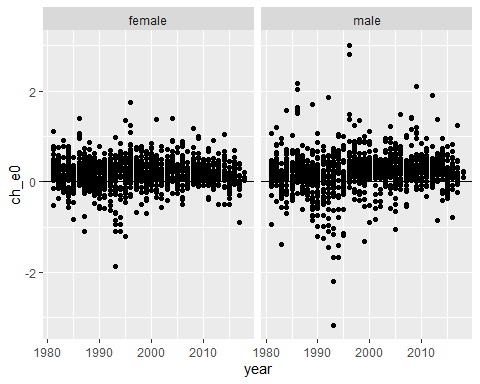
\includegraphics{devils_advocacy_files/figure-latex/unnamed-chunk-7-1.pdf}

This first observation provides very slight support for the hypothesis
that there was a post 2008 slowdown. However, it appears to provide
slightly stronger support for a slowdown in females than males. This
does not appear immediately consonant with the most plausible mechanisms
for a recessionary `bump' in life expectancy, which may be expected to
lead to greater improvements in males than females, as most of the
pathogenic behaviours that a fall in discretionary spend may be assumed
to curtail generally tend to affect male mortality hazards (due to
higher baseline risks) than female mortality hazards. (A converse case
could also be made, however: the effect of a recession can be expected
to reduce discretionary spend, leading to faster rates of improvement in
males than females, as males had previously converted more of their
discretionary spend into pathogenic health behaviours; but also the
effect of a recession can be expected to lead to more unemployment and
under-employment, adversely affecting wellbeing in both genders, which
in males tends to get converted into despair-related mortality, in
particular drug-related deaths and suicide, at a higher rate than in
females. There are threfore mechanisms by which a recession could lead
to an expansion or a contraction in gender differences in mortality, and
the above differences in schedules, based on a single obervation, are
not conclusive in any way.)

The following shows the effect of adding a second observation:

\begin{Shaded}
\begin{Highlighting}[]
\NormalTok{e0_uk_bf }\OperatorTok\StringTok{ }
\StringTok{  }\KeywordTok{filter}\NormalTok{(period }\OperatorTok\StringTok{ }\KeywordTok{c}\NormalTok{(}\StringTok{"2008-09"}\NormalTok{, }\StringTok{"2008-10"}\NormalTok{)) }\OperatorTok\StringTok{ }
\StringTok{  }\KeywordTok{mutate}\NormalTok{(}\DataTypeTok{perc =} \DecValTok{100} \OperatorTok{*}\StringTok{ }\NormalTok{perc) }\OperatorTok\StringTok{ }
\StringTok{  }\KeywordTok{ggplot}\NormalTok{(}\KeywordTok{aes}\NormalTok{(}\DataTypeTok{x =}\NormalTok{ perc, }\DataTypeTok{y =}\NormalTok{ bayes_factor, }\DataTypeTok{alpha =}\NormalTok{ period)) }\OperatorTok{+}
\StringTok{  }\KeywordTok{geom_line}\NormalTok{() }\OperatorTok{+}\StringTok{ }
\StringTok{  }\KeywordTok{geom_ribbon}\NormalTok{(}\KeywordTok{aes}\NormalTok{(}
      \DataTypeTok{ymin =} \KeywordTok{ifelse}\NormalTok{(is_pos, }\DecValTok{1}\NormalTok{, bayes_factor), }
      \DataTypeTok{ymax =} \KeywordTok{ifelse}\NormalTok{(is_pos, bayes_factor, }\DecValTok{1}\NormalTok{), }
      \DataTypeTok{x =}\NormalTok{ perc, }\DataTypeTok{group =} \KeywordTok{paste0}\NormalTok{(is_pos, period),}
      \DataTypeTok{fill =}\NormalTok{ is_pos}
\NormalTok{    ), }
              \DataTypeTok{data =}\NormalTok{ e0_uk_bf }\OperatorTok\StringTok{ }
\StringTok{                }\KeywordTok{filter}\NormalTok{(period }\OperatorTok\StringTok{ }\KeywordTok{c}\NormalTok{(}\StringTok{"2008-09"}\NormalTok{, }\StringTok{"2008-10"}\NormalTok{)) }\OperatorTok\StringTok{ }
\StringTok{                }\KeywordTok{mutate}\NormalTok{(}\DataTypeTok{perc =} \DecValTok{100} \OperatorTok{*}\StringTok{ }\NormalTok{perc) }\OperatorTok
\StringTok{                }\KeywordTok{mutate}\NormalTok{(}\DataTypeTok{is_pos =}\NormalTok{ bayes_factor }\OperatorTok{>}\StringTok{ }\DecValTok{1}\NormalTok{),}
              \DataTypeTok{inherit.aes =} \OtherTok{FALSE}\NormalTok{, }\DataTypeTok{alpha =} \FloatTok{0.2}\NormalTok{) }\OperatorTok{+}\StringTok{ }
\StringTok{  }\KeywordTok{facet_wrap}\NormalTok{(}\OperatorTok{~}\NormalTok{sex) }\OperatorTok{+}
\StringTok{  }\KeywordTok{scale_y_continuous}\NormalTok{(}\DataTypeTok{limits =} \KeywordTok{c}\NormalTok{(}\FloatTok{0.999}\NormalTok{, }\FloatTok{1.005}\NormalTok{), }
                     \DataTypeTok{breaks =} \KeywordTok{seq}\NormalTok{(}\FloatTok{0.999}\NormalTok{, }\FloatTok{1.0050}\NormalTok{, }\DataTypeTok{by =} \FloatTok{0.001}\NormalTok{)}
                       
\NormalTok{                       ) }\OperatorTok{+}
\StringTok{  }\KeywordTok{scale_alpha_discrete}\NormalTok{(}\StringTok{"Period"}\NormalTok{, }\DataTypeTok{range =} \KeywordTok{c}\NormalTok{(}\FloatTok{0.5}\NormalTok{, }\DecValTok{1}\NormalTok{), }\DataTypeTok{breaks =} \KeywordTok{c}\NormalTok{(}\StringTok{"2008-09"}\NormalTok{, }\StringTok{"2008-10"}\NormalTok{)) }\OperatorTok{+}
\StringTok{  }\KeywordTok{geom_hline}\NormalTok{(}\DataTypeTok{yintercept =} \DecValTok{1}\NormalTok{) }\OperatorTok{+}\StringTok{ }
\StringTok{  }\KeywordTok{labs}\NormalTok{(}
    \DataTypeTok{x =} \StringTok{"Percentage of previous improvement"}\NormalTok{,}
    \DataTypeTok{y =} \StringTok{"Bayes Factor}\CharTok{\textbackslash{}n}\StringTok{(>1 means support for Alternative Hypothesis"}\NormalTok{,}
    \DataTypeTok{title =} \StringTok{"Bayes Factor for various proposed levels of slowdown"}\NormalTok{,}
    \DataTypeTok{subtitle =} \StringTok{"Based on periods 2008-09, and 2008-10"}
\NormalTok{  ) }\OperatorTok{+}
\StringTok{  }\KeywordTok{guides}\NormalTok{(}\DataTypeTok{fill =} \OtherTok{FALSE}\NormalTok{)}
\end{Highlighting}
\end{Shaded}

\begin{verbatim}
## Warning: Using alpha for a discrete variable is not advised.
\end{verbatim}

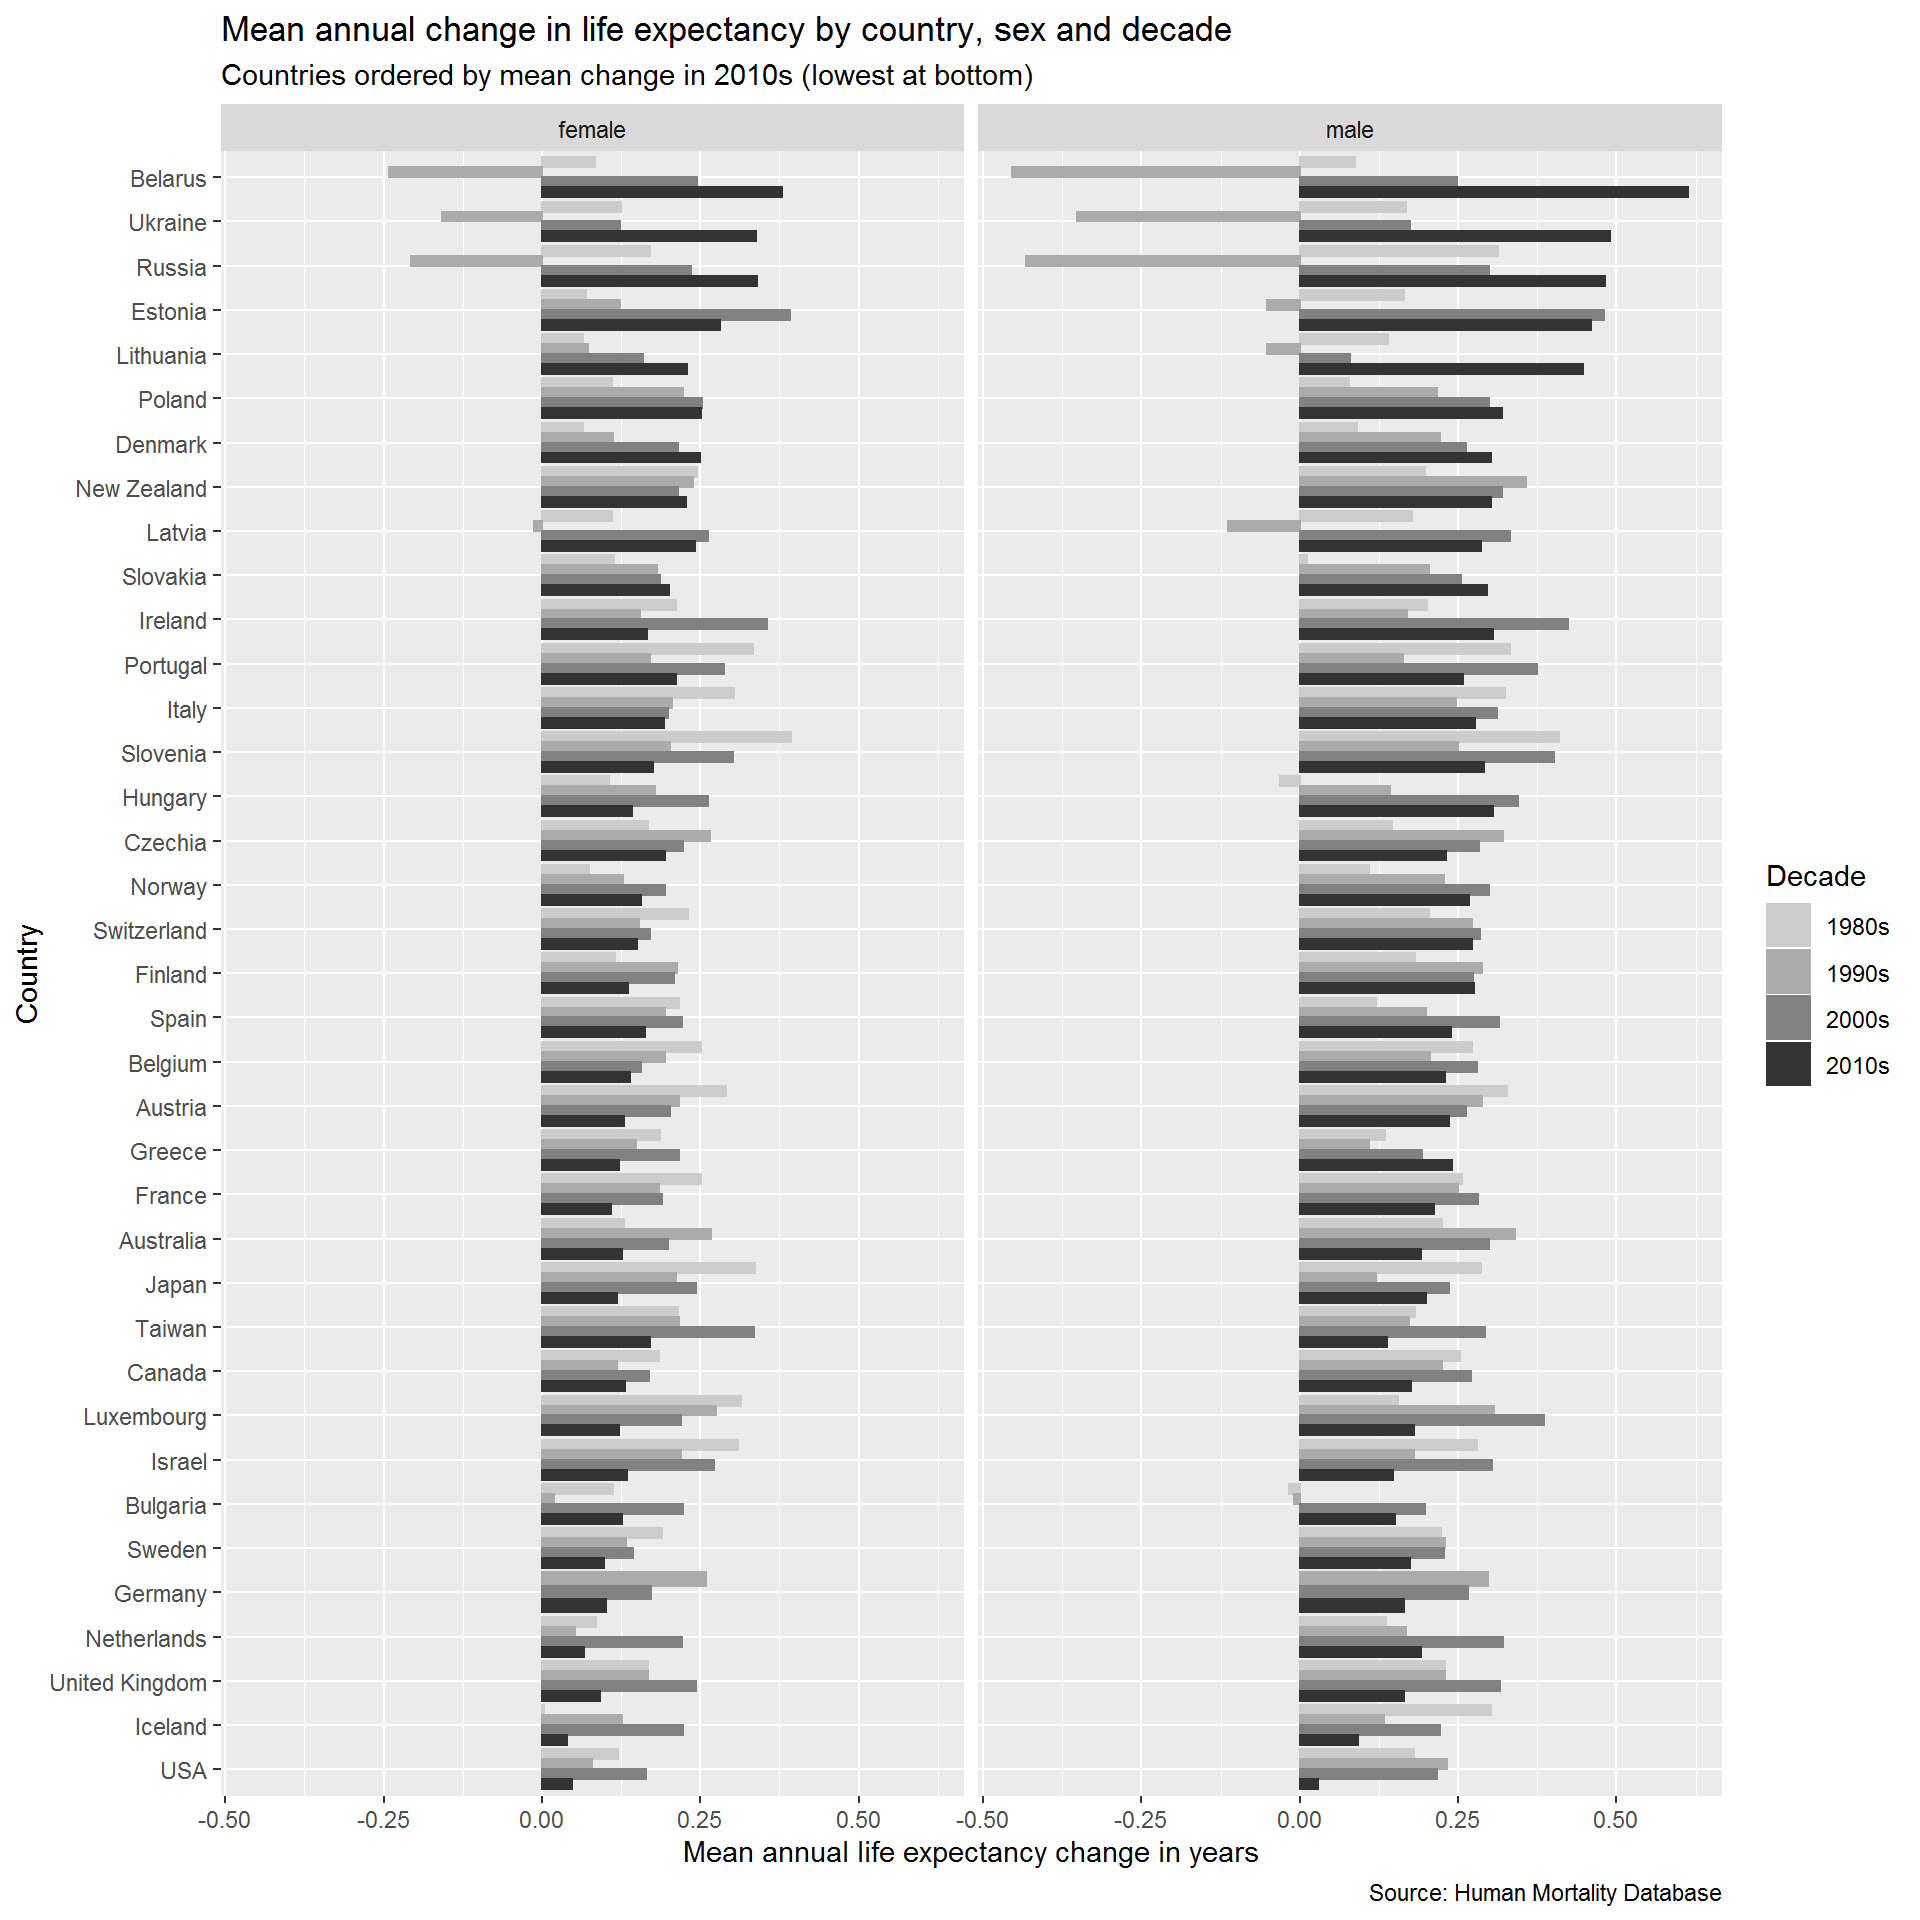
\includegraphics{devils_advocacy_files/figure-latex/unnamed-chunk-8-1.pdf}

With two observations, the support for any kind of GFC Bump has
decreased, and the most likely quantity of the `bump' has decreased -
for females and total - as well. This might be expected if the Bump were
inherently transient in nature, but if it were then this undermines the
broader argument of the GFC Bump interpretation. Namely, that the effect
of the bump on life expectancy were long enough to give the impression
that a return to typical rates of improvement looks like a Slowdown.

The following figure adds the third observation in the series:

\begin{Shaded}
\begin{Highlighting}[]
\NormalTok{e0_uk_bf }\OperatorTok\StringTok{ }
\StringTok{  }\KeywordTok{filter}\NormalTok{(period }\OperatorTok\StringTok{ }\KeywordTok{c}\NormalTok{(}\StringTok{"2008-09"}\NormalTok{, }\StringTok{"2008-10"}\NormalTok{, }\StringTok{"2008-11"}\NormalTok{)) }\OperatorTok\StringTok{ }
\StringTok{  }\KeywordTok{mutate}\NormalTok{(}\DataTypeTok{perc =} \DecValTok{100} \OperatorTok{*}\StringTok{ }\NormalTok{perc) }\OperatorTok\StringTok{ }
\StringTok{  }\KeywordTok{ggplot}\NormalTok{(}\KeywordTok{aes}\NormalTok{(}\DataTypeTok{x =}\NormalTok{ perc, }\DataTypeTok{y =}\NormalTok{ bayes_factor, }\DataTypeTok{alpha =}\NormalTok{ period)) }\OperatorTok{+}
\StringTok{  }\KeywordTok{geom_line}\NormalTok{() }\OperatorTok{+}\StringTok{ }
\StringTok{  }\KeywordTok{geom_ribbon}\NormalTok{(}\KeywordTok{aes}\NormalTok{(}
      \DataTypeTok{ymin =} \KeywordTok{ifelse}\NormalTok{(is_pos, }\DecValTok{1}\NormalTok{, bayes_factor), }
      \DataTypeTok{ymax =} \KeywordTok{ifelse}\NormalTok{(is_pos, bayes_factor, }\DecValTok{1}\NormalTok{), }
      \DataTypeTok{x =}\NormalTok{ perc, }\DataTypeTok{group =} \KeywordTok{paste0}\NormalTok{(is_pos, period),}
      \DataTypeTok{fill =}\NormalTok{ is_pos}
\NormalTok{    ), }
              \DataTypeTok{data =}\NormalTok{ e0_uk_bf }\OperatorTok\StringTok{ }
\StringTok{                }\KeywordTok{filter}\NormalTok{(period }\OperatorTok\StringTok{ }\KeywordTok{c}\NormalTok{(}\StringTok{"2008-09"}\NormalTok{, }\StringTok{"2008-10"}\NormalTok{, }\StringTok{"2008-11"}\NormalTok{)) }\OperatorTok\StringTok{ }
\StringTok{                }\KeywordTok{mutate}\NormalTok{(}\DataTypeTok{perc =} \DecValTok{100} \OperatorTok{*}\StringTok{ }\NormalTok{perc) }\OperatorTok
\StringTok{                }\KeywordTok{mutate}\NormalTok{(}\DataTypeTok{is_pos =}\NormalTok{ bayes_factor }\OperatorTok{>}\StringTok{ }\DecValTok{1}\NormalTok{),}
              \DataTypeTok{inherit.aes =} \OtherTok{FALSE}\NormalTok{, }\DataTypeTok{alpha =} \FloatTok{0.2}\NormalTok{) }\OperatorTok{+}\StringTok{ }
\StringTok{  }\KeywordTok{facet_wrap}\NormalTok{(}\OperatorTok{~}\NormalTok{sex) }\OperatorTok{+}
\StringTok{  }\KeywordTok{scale_y_continuous}\NormalTok{(}\DataTypeTok{limits =} \KeywordTok{c}\NormalTok{(}\FloatTok{0.999}\NormalTok{, }\FloatTok{1.005}\NormalTok{), }
                     \DataTypeTok{breaks =} \KeywordTok{seq}\NormalTok{(}\FloatTok{0.999}\NormalTok{, }\FloatTok{1.0050}\NormalTok{, }\DataTypeTok{by =} \FloatTok{0.001}\NormalTok{)}
                       
\NormalTok{                       ) }\OperatorTok{+}
\StringTok{  }\KeywordTok{scale_alpha_discrete}\NormalTok{(}\StringTok{"Period"}\NormalTok{, }\DataTypeTok{range =} \KeywordTok{c}\NormalTok{(}\FloatTok{0.5}\NormalTok{, }\DecValTok{1}\NormalTok{), }\DataTypeTok{breaks =} \KeywordTok{c}\NormalTok{(}\StringTok{"2008-09"}\NormalTok{, }\StringTok{"2008-10"}\NormalTok{, }\StringTok{"2008-11"}\NormalTok{)) }\OperatorTok{+}
\StringTok{  }\KeywordTok{geom_hline}\NormalTok{(}\DataTypeTok{yintercept =} \DecValTok{1}\NormalTok{) }\OperatorTok{+}\StringTok{ }
\StringTok{  }\KeywordTok{labs}\NormalTok{(}
    \DataTypeTok{x =} \StringTok{"Percentage of previous improvement"}\NormalTok{,}
    \DataTypeTok{y =} \StringTok{"Bayes Factor}\CharTok{\textbackslash{}n}\StringTok{(>1 means support for Alternative Hypothesis"}\NormalTok{,}
    \DataTypeTok{title =} \StringTok{"Bayes Factor for various proposed levels of slowdown"}\NormalTok{,}
    \DataTypeTok{subtitle =} \StringTok{"Based on periods 2008-09 to 2008-11"}
\NormalTok{  ) }\OperatorTok{+}
\StringTok{  }\KeywordTok{guides}\NormalTok{(}\DataTypeTok{fill =} \OtherTok{FALSE}\NormalTok{)}
\end{Highlighting}
\end{Shaded}

\begin{verbatim}
## Warning: Using alpha for a discrete variable is not advised.
\end{verbatim}

\includegraphics{devils_advocacy_files/figure-latex/unnamed-chunk-9-1.pdf}

With the addition of this third observation, from 2010-2011, the support
for a Bump has increased again, with no proposed level of improvement up
to 200\% of trend levels being `less likely' than the hypothesis that
there has been no improvement.

The following adds a forth observation, from 2011-2012.

\begin{Shaded}
\begin{Highlighting}[]
\NormalTok{e0_uk_bf }\OperatorTok\StringTok{ }
\StringTok{  }\KeywordTok{filter}\NormalTok{(period }\OperatorTok\StringTok{ }\KeywordTok{c}\NormalTok{(}\StringTok{"2008-09"}\NormalTok{, }\StringTok{"2008-10"}\NormalTok{, }\StringTok{"2008-11"}\NormalTok{, }\StringTok{"2008-12"}\NormalTok{)) }\OperatorTok\StringTok{ }
\StringTok{  }\KeywordTok{mutate}\NormalTok{(}\DataTypeTok{perc =} \DecValTok{100} \OperatorTok{*}\StringTok{ }\NormalTok{perc) }\OperatorTok\StringTok{ }
\StringTok{  }\KeywordTok{ggplot}\NormalTok{(}\KeywordTok{aes}\NormalTok{(}\DataTypeTok{x =}\NormalTok{ perc, }\DataTypeTok{y =}\NormalTok{ bayes_factor, }\DataTypeTok{alpha =}\NormalTok{ period)) }\OperatorTok{+}
\StringTok{  }\KeywordTok{geom_line}\NormalTok{() }\OperatorTok{+}\StringTok{ }
\StringTok{  }\KeywordTok{geom_ribbon}\NormalTok{(}\KeywordTok{aes}\NormalTok{(}
      \DataTypeTok{ymin =} \KeywordTok{ifelse}\NormalTok{(is_pos, }\DecValTok{1}\NormalTok{, bayes_factor), }
      \DataTypeTok{ymax =} \KeywordTok{ifelse}\NormalTok{(is_pos, bayes_factor, }\DecValTok{1}\NormalTok{), }
      \DataTypeTok{x =}\NormalTok{ perc, }\DataTypeTok{group =} \KeywordTok{paste0}\NormalTok{(is_pos, period),}
      \DataTypeTok{fill =}\NormalTok{ is_pos}
\NormalTok{    ), }
              \DataTypeTok{data =}\NormalTok{ e0_uk_bf }\OperatorTok\StringTok{ }
\StringTok{                }\KeywordTok{filter}\NormalTok{(period }\OperatorTok\StringTok{ }\KeywordTok{c}\NormalTok{(}\StringTok{"2008-09"}\NormalTok{, }\StringTok{"2008-10"}\NormalTok{, }\StringTok{"2008-11"}\NormalTok{, }\StringTok{"2008-12"}\NormalTok{)) }\OperatorTok\StringTok{ }
\StringTok{                }\KeywordTok{mutate}\NormalTok{(}\DataTypeTok{perc =} \DecValTok{100} \OperatorTok{*}\StringTok{ }\NormalTok{perc) }\OperatorTok
\StringTok{                }\KeywordTok{mutate}\NormalTok{(}\DataTypeTok{is_pos =}\NormalTok{ bayes_factor }\OperatorTok{>}\StringTok{ }\DecValTok{1}\NormalTok{),}
              \DataTypeTok{inherit.aes =} \OtherTok{FALSE}\NormalTok{, }\DataTypeTok{alpha =} \FloatTok{0.2}\NormalTok{) }\OperatorTok{+}\StringTok{ }
\StringTok{  }\KeywordTok{facet_wrap}\NormalTok{(}\OperatorTok{~}\NormalTok{sex) }\OperatorTok{+}
\StringTok{  }\KeywordTok{scale_y_continuous}\NormalTok{(}\DataTypeTok{limits =} \KeywordTok{c}\NormalTok{(}\FloatTok{0.998}\NormalTok{, }\FloatTok{1.005}\NormalTok{), }
                     \DataTypeTok{breaks =} \KeywordTok{seq}\NormalTok{(}\FloatTok{0.998}\NormalTok{, }\FloatTok{1.0050}\NormalTok{, }\DataTypeTok{by =} \FloatTok{0.001}\NormalTok{)}
                       
\NormalTok{                       ) }\OperatorTok{+}
\StringTok{  }\KeywordTok{scale_alpha_discrete}\NormalTok{(}\StringTok{"Period"}\NormalTok{, }\DataTypeTok{range =} \KeywordTok{c}\NormalTok{(}\FloatTok{0.5}\NormalTok{, }\DecValTok{1}\NormalTok{), }\DataTypeTok{breaks =} \KeywordTok{c}\NormalTok{(}\StringTok{"2008-09"}\NormalTok{, }\StringTok{"2008-10"}\NormalTok{, }\StringTok{"2008-11"}\NormalTok{, }\StringTok{"2008-12"}\NormalTok{)) }\OperatorTok{+}
\StringTok{  }\KeywordTok{geom_hline}\NormalTok{(}\DataTypeTok{yintercept =} \DecValTok{1}\NormalTok{) }\OperatorTok{+}\StringTok{ }
\StringTok{  }\KeywordTok{labs}\NormalTok{(}
    \DataTypeTok{x =} \StringTok{"Percentage of previous improvement"}\NormalTok{,}
    \DataTypeTok{y =} \StringTok{"Bayes Factor}\CharTok{\textbackslash{}n}\StringTok{(>1 means support for Alternative Hypothesis"}\NormalTok{,}
    \DataTypeTok{title =} \StringTok{"Bayes Factor for various proposed levels of slowdown"}\NormalTok{,}
    \DataTypeTok{subtitle =} \StringTok{"Based on periods 2008-09 to 2008-12"}
\NormalTok{  ) }\OperatorTok{+}
\StringTok{  }\KeywordTok{guides}\NormalTok{(}\DataTypeTok{fill =} \OtherTok{FALSE}\NormalTok{)}
\end{Highlighting}
\end{Shaded}

\begin{verbatim}
## Warning: Using alpha for a discrete variable is not advised.
\end{verbatim}

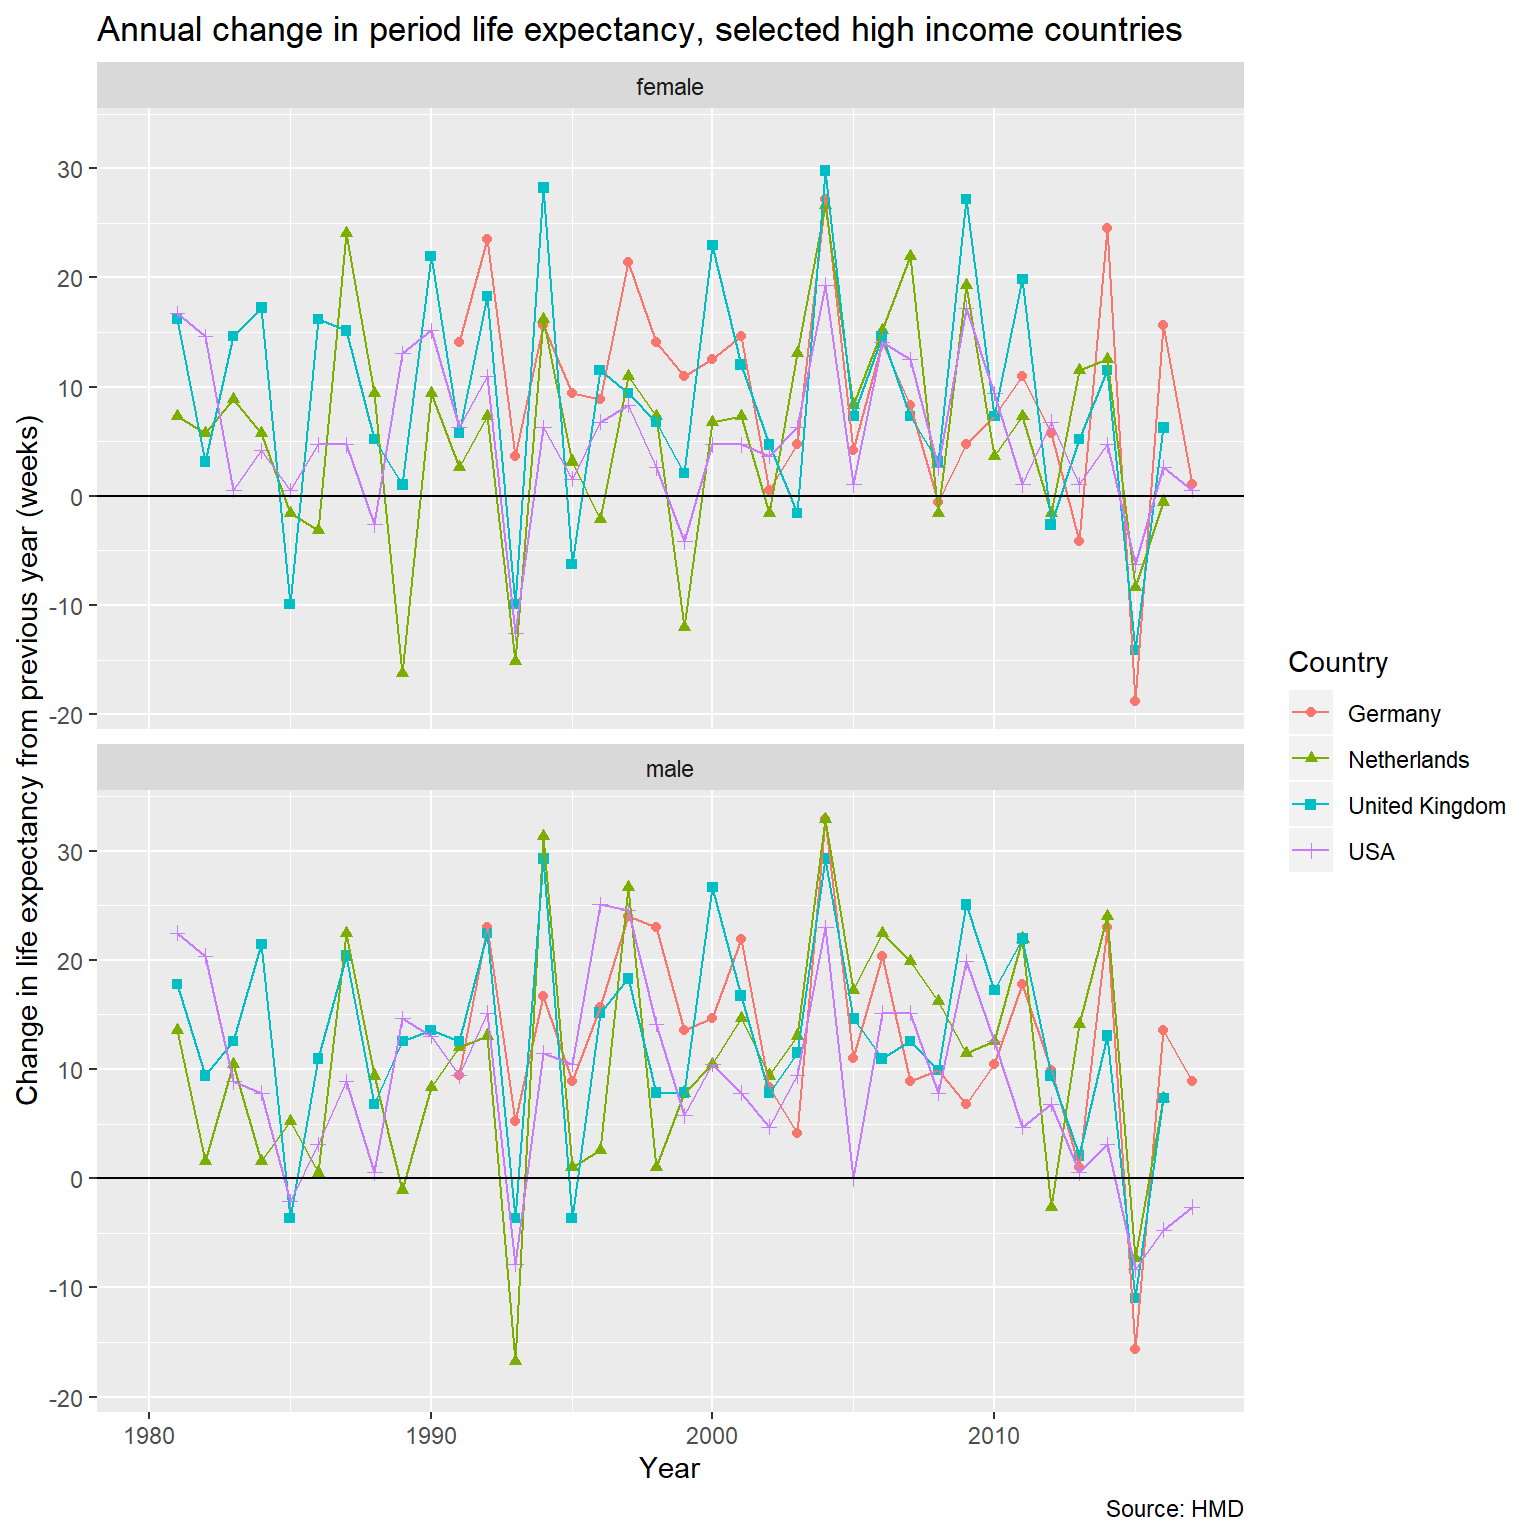
\includegraphics{devils_advocacy_files/figure-latex/unnamed-chunk-10-1.pdf}

With this forth observation, the support for the Bump interpretation has
decreased, especially for females. The most likely level of improvement
has also fallen, and many higher rates of proposed improvement are now
less likely than the No Improvement hypothesis. (Red region below 1.000.
The scale has been adjusted to allow the full schedule to be shown)

Finally, the following shows the effect of incorporating the fifth
observation, from 2012-2013.

\begin{Shaded}
\begin{Highlighting}[]
\NormalTok{e0_uk_bf }\OperatorTok\StringTok{ }
\StringTok{  }\KeywordTok{filter}\NormalTok{(period }\OperatorTok\StringTok{ }\KeywordTok{c}\NormalTok{(}\StringTok{"2008-09"}\NormalTok{, }\StringTok{"2008-10"}\NormalTok{, }\StringTok{"2008-11"}\NormalTok{, }\StringTok{"2008-12"}\NormalTok{, }\StringTok{"2008-13"}\NormalTok{)) }\OperatorTok\StringTok{ }
\StringTok{  }\KeywordTok{mutate}\NormalTok{(}\DataTypeTok{perc =} \DecValTok{100} \OperatorTok{*}\StringTok{ }\NormalTok{perc) }\OperatorTok\StringTok{ }
\StringTok{  }\KeywordTok{ggplot}\NormalTok{(}\KeywordTok{aes}\NormalTok{(}\DataTypeTok{x =}\NormalTok{ perc, }\DataTypeTok{y =}\NormalTok{ bayes_factor, }\DataTypeTok{alpha =}\NormalTok{ period)) }\OperatorTok{+}
\StringTok{  }\KeywordTok{geom_line}\NormalTok{() }\OperatorTok{+}\StringTok{ }
\StringTok{  }\KeywordTok{geom_ribbon}\NormalTok{(}\KeywordTok{aes}\NormalTok{(}
      \DataTypeTok{ymin =} \KeywordTok{ifelse}\NormalTok{(is_pos, }\DecValTok{1}\NormalTok{, bayes_factor), }
      \DataTypeTok{ymax =} \KeywordTok{ifelse}\NormalTok{(is_pos, bayes_factor, }\DecValTok{1}\NormalTok{), }
      \DataTypeTok{x =}\NormalTok{ perc, }\DataTypeTok{group =} \KeywordTok{paste0}\NormalTok{(is_pos, period),}
      \DataTypeTok{fill =}\NormalTok{ is_pos}
\NormalTok{    ), }
              \DataTypeTok{data =}\NormalTok{ e0_uk_bf }\OperatorTok\StringTok{ }
\StringTok{                }\KeywordTok{filter}\NormalTok{(period }\OperatorTok\StringTok{ }\KeywordTok{c}\NormalTok{(}\StringTok{"2008-09"}\NormalTok{, }\StringTok{"2008-10"}\NormalTok{, }\StringTok{"2008-11"}\NormalTok{, }\StringTok{"2008-12"}\NormalTok{, }\StringTok{"2008-13"}\NormalTok{)) }\OperatorTok\StringTok{ }
\StringTok{                }\KeywordTok{mutate}\NormalTok{(}\DataTypeTok{perc =} \DecValTok{100} \OperatorTok{*}\StringTok{ }\NormalTok{perc) }\OperatorTok
\StringTok{                }\KeywordTok{mutate}\NormalTok{(}\DataTypeTok{is_pos =}\NormalTok{ bayes_factor }\OperatorTok{>}\StringTok{ }\DecValTok{1}\NormalTok{),}
              \DataTypeTok{inherit.aes =} \OtherTok{FALSE}\NormalTok{, }\DataTypeTok{alpha =} \FloatTok{0.2}\NormalTok{) }\OperatorTok{+}\StringTok{ }
\StringTok{  }\KeywordTok{facet_wrap}\NormalTok{(}\OperatorTok{~}\NormalTok{sex) }\OperatorTok{+}
\StringTok{  }\KeywordTok{scale_y_continuous}\NormalTok{(}\DataTypeTok{limits =} \KeywordTok{c}\NormalTok{(}\FloatTok{0.996}\NormalTok{, }\FloatTok{1.005}\NormalTok{), }
                     \DataTypeTok{breaks =} \KeywordTok{seq}\NormalTok{(}\FloatTok{0.996}\NormalTok{, }\FloatTok{1.0050}\NormalTok{, }\DataTypeTok{by =} \FloatTok{0.001}\NormalTok{)}
                       
\NormalTok{                       ) }\OperatorTok{+}
\StringTok{  }\KeywordTok{scale_alpha_discrete}\NormalTok{(}\StringTok{"Period"}\NormalTok{, }\DataTypeTok{range =} \KeywordTok{c}\NormalTok{(}\FloatTok{0.5}\NormalTok{, }\DecValTok{1}\NormalTok{), }\DataTypeTok{breaks =} \KeywordTok{c}\NormalTok{(}\StringTok{"2008-09"}\NormalTok{, }\StringTok{"2008-10"}\NormalTok{, }\StringTok{"2008-11"}\NormalTok{, }\StringTok{"2008-12"}\NormalTok{, }\StringTok{"2008-13"}\NormalTok{)) }\OperatorTok{+}
\StringTok{  }\KeywordTok{geom_hline}\NormalTok{(}\DataTypeTok{yintercept =} \DecValTok{1}\NormalTok{) }\OperatorTok{+}\StringTok{ }
\StringTok{  }\KeywordTok{labs}\NormalTok{(}
    \DataTypeTok{x =} \StringTok{"Percentage of previous improvement"}\NormalTok{,}
    \DataTypeTok{y =} \StringTok{"Bayes Factor}\CharTok{\textbackslash{}n}\StringTok{(>1 means support for Alternative Hypothesis"}\NormalTok{,}
    \DataTypeTok{title =} \StringTok{"Bayes Factor for various proposed levels of slowdown"}\NormalTok{,}
    \DataTypeTok{subtitle =} \StringTok{"Based on periods 2008-09 to 2008-13"}
\NormalTok{  ) }\OperatorTok{+}
\StringTok{  }\KeywordTok{guides}\NormalTok{(}\DataTypeTok{fill =} \OtherTok{FALSE}\NormalTok{)}
\end{Highlighting}
\end{Shaded}

\begin{verbatim}
## Warning: Using alpha for a discrete variable is not advised.
\end{verbatim}

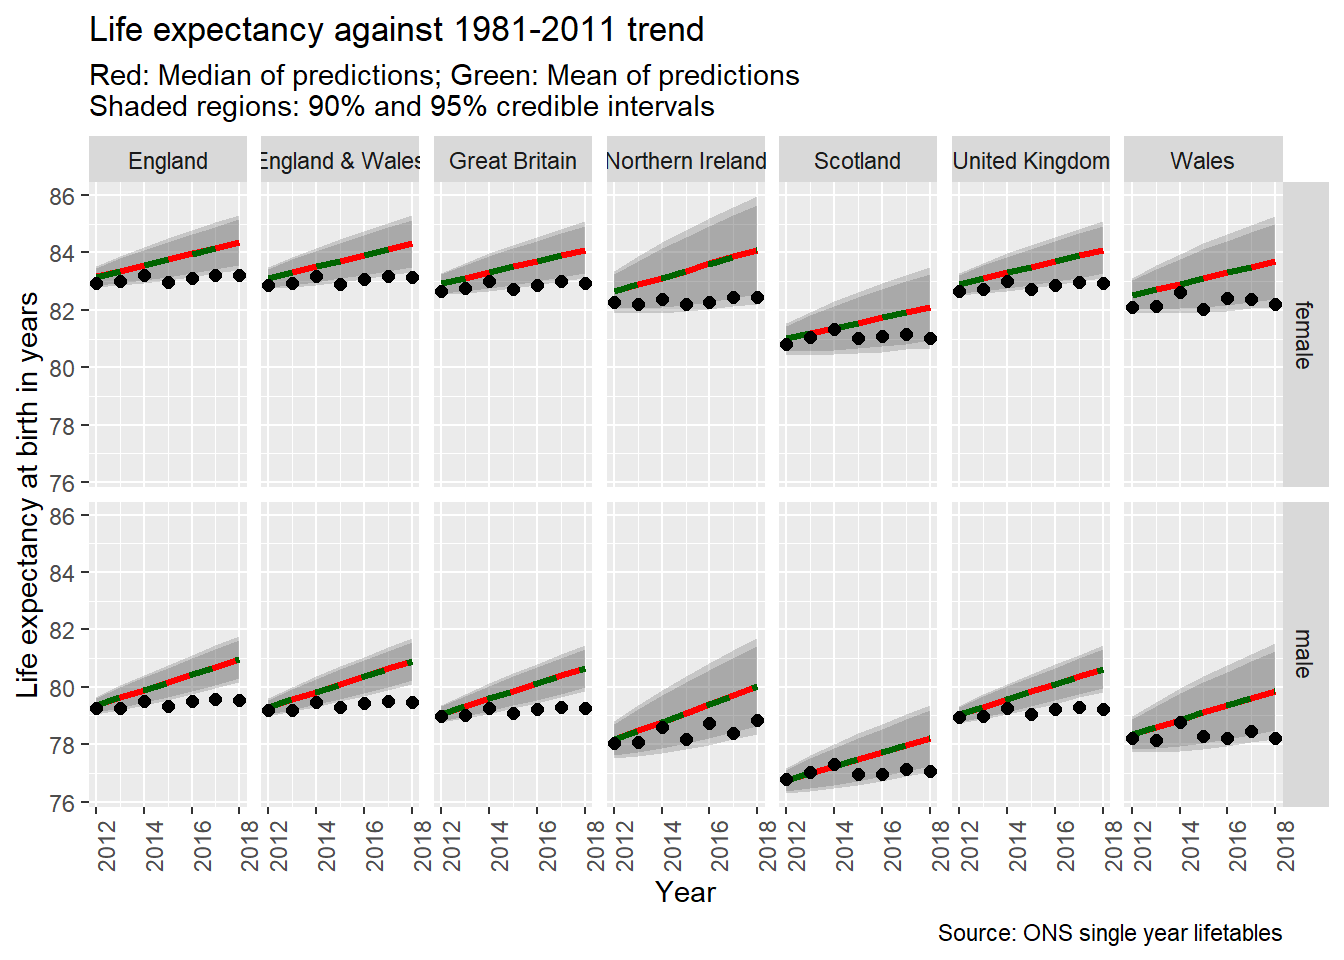
\includegraphics{devils_advocacy_files/figure-latex/unnamed-chunk-11-1.pdf}
The lower part of the scale has been expanded further because the lower
bounds of the estimated Bayes Factors is even lower. With five full
observations, there now appears to be very little evidence of a
sustained GFC Bump.

The final figure shows only the schedule based on all five observations.

\begin{Shaded}
\begin{Highlighting}[]
\NormalTok{e0_uk_bf }\OperatorTok\StringTok{ }
\StringTok{  }\KeywordTok{filter}\NormalTok{(period }\OperatorTok{==}\StringTok{ "2008-13"}\NormalTok{) }\OperatorTok\StringTok{ }
\StringTok{  }\KeywordTok{mutate}\NormalTok{(}\DataTypeTok{perc =} \DecValTok{100} \OperatorTok{*}\StringTok{ }\NormalTok{perc) }\OperatorTok\StringTok{ }
\StringTok{  }\KeywordTok{ggplot}\NormalTok{(}\KeywordTok{aes}\NormalTok{(}\DataTypeTok{x =}\NormalTok{ perc, }\DataTypeTok{y =}\NormalTok{ bayes_factor)) }\OperatorTok{+}
\StringTok{  }\KeywordTok{geom_line}\NormalTok{() }\OperatorTok{+}\StringTok{ }
\StringTok{  }\KeywordTok{geom_ribbon}\NormalTok{(}\KeywordTok{aes}\NormalTok{(}
      \DataTypeTok{ymin =} \KeywordTok{ifelse}\NormalTok{(is_pos, }\DecValTok{1}\NormalTok{, bayes_factor), }
      \DataTypeTok{ymax =} \KeywordTok{ifelse}\NormalTok{(is_pos, bayes_factor, }\DecValTok{1}\NormalTok{), }
      \DataTypeTok{x =}\NormalTok{ perc, }\DataTypeTok{group =} \KeywordTok{paste0}\NormalTok{(is_pos, period),}
      \DataTypeTok{fill =}\NormalTok{ is_pos}
\NormalTok{    ), }
              \DataTypeTok{data =}\NormalTok{ e0_uk_bf }\OperatorTok\StringTok{ }
\StringTok{                }\KeywordTok{filter}\NormalTok{(period }\OperatorTok{==}\StringTok{ "2008-13"}\NormalTok{) }\OperatorTok\StringTok{ }
\StringTok{                }\KeywordTok{mutate}\NormalTok{(}\DataTypeTok{perc =} \DecValTok{100} \OperatorTok{*}\StringTok{ }\NormalTok{perc) }\OperatorTok
\StringTok{                }\KeywordTok{mutate}\NormalTok{(}\DataTypeTok{is_pos =}\NormalTok{ bayes_factor }\OperatorTok{>}\StringTok{ }\DecValTok{1}\NormalTok{),}
              \DataTypeTok{inherit.aes =} \OtherTok{FALSE}\NormalTok{, }\DataTypeTok{alpha =} \FloatTok{0.2}\NormalTok{) }\OperatorTok{+}\StringTok{ }
\StringTok{  }\KeywordTok{facet_wrap}\NormalTok{(}\OperatorTok{~}\NormalTok{sex) }\OperatorTok{+}
\StringTok{  }\KeywordTok{scale_y_continuous}\NormalTok{(}\DataTypeTok{limits =} \KeywordTok{c}\NormalTok{(}\FloatTok{0.996}\NormalTok{, }\FloatTok{1.005}\NormalTok{), }
                     \DataTypeTok{breaks =} \KeywordTok{seq}\NormalTok{(}\FloatTok{0.996}\NormalTok{, }\FloatTok{1.0050}\NormalTok{, }\DataTypeTok{by =} \FloatTok{0.001}\NormalTok{)}
                       
\NormalTok{                       ) }\OperatorTok{+}
\StringTok{  }\KeywordTok{geom_hline}\NormalTok{(}\DataTypeTok{yintercept =} \DecValTok{1}\NormalTok{) }\OperatorTok{+}\StringTok{ }
\StringTok{  }\KeywordTok{labs}\NormalTok{(}
    \DataTypeTok{x =} \StringTok{"Percentage of previous improvement"}\NormalTok{,}
    \DataTypeTok{y =} \StringTok{"Bayes Factor}\CharTok{\textbackslash{}n}\StringTok{(>1 means support for Alternative Hypothesis"}\NormalTok{,}
    \DataTypeTok{title =} \StringTok{"Bayes Factor for various proposed levels of slowdown"}\NormalTok{,}
    \DataTypeTok{subtitle =} \StringTok{"Based on periods 2008-09 to 2008-13"}
\NormalTok{  ) }\OperatorTok{+}
\StringTok{  }\KeywordTok{guides}\NormalTok{(}\DataTypeTok{fill =} \OtherTok{FALSE}\NormalTok{)}
\end{Highlighting}
\end{Shaded}

\includegraphics{devils_advocacy_files/figure-latex/unnamed-chunk-12-1.pdf}

\section{Discussion}\label{discussion}

With five continuous observations, the evidence is against a GFC Bump
interpetation of the UK life expectancy series since 1990. The Bayes
Factor maximises at around a 15\% improvement rate, with a maximum Bayes
Factor of around 1.0001. This compares with a Bayes Factor for the
Slowdown Hypothesis, also based on five observations, which maximises at
around 1.003, when a slowdown to around 20\% of pre-slowdown levels is
assumed.

As the two interpretations are not being directly compared, and the Null
hypotheses considered in both interpretations are different, it is
probably theoretically inappropriate to conclude, on the basis of this,
that the data provide around 30 times (1.003 / 1.0001) more support for
the Slowdown interpretation than the GFC Bump interpetation. However,
the results of this exercise in `Devil's Advocacy' do not appear to
provide a strong case for preferring the GFC Bump interpretation over
the Slowdown interpretation of recent UK life expectancy trends in a
longer-term context. The evidence does not appear to be `moot' with
regards to how convincing these two interpretations are. Put another
way, the data are not a Duck-Rabbit, which can be interpreted equally
plausibly as either a `Duck' (GFC Bump) or a `Rabbit' (Slowdown).


\end{document}
